\documentclass[twoside,a4paper]{article}

\usepackage{graphicx}
\usepackage{url}
\usepackage{verbatim}
\usepackage{tikz}
\usetikzlibrary{arrows,shapes}

\title{ Multimodal recommender engine based on Apache Mahout and Apache Solr }
\author{
	Author \\
	Lukas Hofmaier \\
	lukas.hofmaier@hsr.ch
 	\and
	Supervisors \\
        Hansj''org Huser
}
\date{
	\textsc{University of Applied Sciences Rapperswil}\\
	Project Thesis,
	\today
}
\begin{document}
\maketitle
\tableofcontents

\section{Introduction}
\label{sec:intro}

Recommender systems help consumers to discover unknown articles from an overwhelming set of choices by suggesting them a list of items that are likely to be appealing to them. The recommended items should match the user's personal taste.

For instance, they help users of an on-demand movie provider to find previously unknown and interesting movies. Such a provider may offer 100'000 different titles. It is not feasible for a user to check every movie separately in order to decide if he likes it or not. A recommender engine supports users by presenting them a list of movie recommendations. It predicts the user's \gls{preference} for each movie and shows him a list of movies with the highest predicted score. The list of recommendations is referred to as \gls{topn}. For example, if a user has purchased the movies "Terminator 2" and "Transformers" the recommender engine might present him a list of other similar action movies like ``Matrix'' or ``Iron Man''. 
 
Recommender systems have become very common in recent years. E-commerce sites that deploy a recommender engine can have an increase in sales of 8-13 percent.\footnote{http://www.practicalecommerce.com/articles/1942-10-Questions-on-Product-Recommendations}

\subsection{Overview of recommender strategies}
\label{sec:strategies}

A trivial solution to the recommender problem would be to sort all items by their popularity or average rating in descending order and then suggesting the user the top $N$ items of that sorted list. Recommender systems based on this approach are called non-personalized. Non-personalized \glspl{topn} do not involve computationally expensive procedures and are easy to implement but they suggest all users the same items. The web site www.imdb.com is an example for a non-personalized recommender. It shows the user a list of movies sorted by the average rating score.
 The recommender described in this report is a personalized recommender that creates an individual list of recommendation for every user.

There are different strategies to create personalized \glspl{topn} \cite{jannach11}. Figure \ref{fig:overview} shows an overview of some possible techniques.

\tikzset{
  basic/.style  = {draw, text width=3cm, drop shadow, font=\sffamily, rectangle},
  root/.style   = {basic, rounded corners=2pt, thin, align=center,
                   fill=green!30},
  level 2/.style = {basic, rounded corners=6pt, thin,align=center, fill=green!60,
                   text width=8em, edge from parent/.style={->,draw,color=black},>=latex},
  level 3/.style = {basic, thin, align=left, fill=pink!60, text width=8.5em}
}
\begin{figure}
  \centering
\begin{tikzpicture}[
  level 1/.style={sibling distance=50mm},
  edge from parent/.style={->,draw},
  >=latex]

% root of the the initial tree, level 1
\node[root] {Recommender strategy}
% The first level, as children of the initial tree
  child {node[root] (c1) {Non-personalized}}
  child {node[root] (c2) {personalized}
    child {node[level 2] (c21) {Collaborative filtering}
      child {node[level 2] (c2111) {Neighborhood based}}
      child {node[level 2] (c2112) {Latent factor approach}}}
    child {node[level 2] (c22) {\gls{content} filtering}}};
  
% The second level, relatively positioned nodes
\begin{scope}[every node/.style={level 3}]

\node [below of = c2111, xshift=15pt] (c211) {Pearson Correlation};
\node [below of = c211] (c212) {Cosine similarity};
\node [below of = c212] (c213) {LLR ratio};

\node [below of = c2112, xshift=15pt] (c21121) {Gradient descent};
\node [below of = c21121] (c21122) {Least Square};

\end{scope}

% lines from each level 1 node to every one of its "children"

\foreach \value in {1,...,3}
  \draw[->] (c2111.195) |- (c21\value.west);

\foreach \value in {1,...,2}
  \draw[->] (c2112.195) |- (c2112\value.west);

\end{tikzpicture}
    \caption{Overview of some common recommender strategies}
\label{fig:overview}
\end{figure}


\begin{description}
\item[Collaborative Filtering] This strategy is only based on past user behavior. Such behavior include explicit user ratings or other user activities like purchases, likes and clicks. For example, a recommender engine based on collaborative filtering uses the ratings of all users to compute the similarity between all items. 
It requires no domain knowledge. Recommender engines based on collaborative filtering do not care what the items are and what attributes they have. This can be an advantage because the same technique can be applied to different domains and different types of items. 

User preferences will change over time. Another advantage is that collaborative filtering will update the model automatically as it is exposed to new user histories. The systems learns.
Further collaborative filtering algorithms can be divided in two different approaches.
\begin{description}
\item[Neighborhood based] Neighborhood models are based on the similarity among users or items. For instance, two items are similar because they have similar ratings of the same users. The set of items that are similar to a particular item $i$ is called the neighborhood of $i$. In order to predict a unknown preference for an item $i$ the recommender computes the nearest neighbors of $i$ and considers the users past ratings for the similar items. This approach was used by Amazon.com according to \cite{Linden}. Neighborhood models can be further divided by their similarity metric (e.g. cosine, log-likelihood ratio).
\item[Latent factor approach] Latent factor approaches model users and items as vectors. The rating of a user on an item is predicted by computing the inner product between the related latent factor vectors. The recommender problem is reduced to the optimization problem of finding the best vectors with respect to a training set.
\end{description}
\item[\gls{content} filtering] \gls{content} recommendation techniques use attributes of items in order to predict preferences of users. For example, a movie can be described by \glspl{tag}. A user profile indicates the type of items a user likes. These algorithms recommend items that are similar to the user profile. The profile could be built from the user's past actions.
\end{description}

This report describes a personalized recommender that uses a combination of collaborative filtering and content-based filtering. In order to compute similarities among items it uses both; past user actions and \glspl{tag} associated with items. Hence it is a hybrid recommender system.

\subsection{Why is it difficult to build a recommender engine?}

To make a rationally choice which strategy to use for the job at hand is difficult and requires a strong mathematical background. According to \cite{Dunning14} the process of designing an advanced and accurate recommender engine requires a team of highly trained engineers and data scientists. The process requires to try a huge collection of algorithms for each problem and selecting the algorithm that gives the best result. This is too expensive for small companies. Apart from choosing the strategy there are several other challenges in building a recommender engine.

\begin{itemize}
\item Collaborative filtering algorithms are based on collecting a large amount of past user preference data. Most techniques use explicit user ratings. For instance, users are invited to rate items on a scale from 1 to 5. Only a small subset of users rate a small subset of items. This leads to very few ratings and these ratings represent only users who like to rate.

\item When dealing with huge data sets, the calculation of the similarities or the latent factor vector is computationally expensive. Either a large amount of computation power is necessary or the computation of a \gls{topn} takes too long.
\end{itemize}

\subsection{The design goals of a practical recommender}
\label{sec:practical}

In order make the development of a recommender engine easier and cost-effective Ted Dunning  proposes in \cite{Dunning14} a simplified, practical approach that provides profitable results and facilitate the processing of large-scale data sets. 

The design proposed by \cite{Dunning14} has the following goals:
\begin{itemize}
\item A small-scale development teams can build a recommender engine.
\item To build the model, the systems uses algorithms that can be computed at scale with a distributed computation framework, such as Apache Hadoop or Apache Spark. 
\item The \gls{topnt} should be fast. Recommendations are generated instantly and online. Computation of similarity and the update of the text search engine is done offline, ahead of time.
\item Use input data that reveals what user want to do. The quality of a recommender depends on the input data that is used to build the model (train the recommender). 
\item Several types (e.g. clicks, views, purchases) of user actions are used to improve recommendations and it is possible to extend the recommender with additional \glspl{indicator}. Many existing collaborative filtering algorithms use only one user activity to model preference \cite{ferrel}. In addition meta data, like \glspl{tag}, are used to improve the accuracy. A recommender that uses a variety of user activities is called a \gls{multimodal} recommender. 
\end{itemize}

To achieve these goals Ted Dunning makes the following suggestions in \cite{Dunning14}.

\begin{itemize}
\item The recommender engine takes user behavior instead of explicit user ratings as input. Because only a small subset of users are willing to rate items and user behavior is the best clue to what they want. Hence the input data should consist of collected user behavior, like clicking or purchasing.

\item Use \gls{coocc} as an \gls{indicator} for similarity. Co-occurrence counts how many times two items appear together in user histories. Among others there are two reason to use \gls{coocc}. 

\begin{itemize}
  \item User behavior interaction are only associations between a user and an item and there is no notion of the association's strength represented as number. This associations are Boolean preferences. It exist or it doesn't exist. Co-occurrence is suitable for Boolean preferences because it does not account for a strength of the interaction. In addition, it can be used to analyze every type of interaction. For instance, we can also count \gls{coocc} of items associated with tags.
  \item Co-occurrence can be computed using the \gls{mapreduce} programming model. Hence the computation of the model can be distributed.
\end{itemize}

\item Use a text retrieval engine to produce the \gls{topn}. Producing a \gls{topn} with a neighborhood based collaborative filtering algorithm is similar to process a document query in a text retrieval system. Because a \gls{rankedretrieval} is a way of finding similar documents according to a query we can use \gls{rankedretrieval} to find similar items to the ones the user already expressed some interest.
 We use similarity indicators based on \gls{coocc} to score every item that matches the query.
The search engine indexes items represented as documents instead of text documents. The fields of these documents contain similar items. The query is composed of items that are associated with the user's past actions which we want to recommend. For instance, if we want to recommend items which the user can purchase then we use his purchase history. 

It is possible to store several indicators as fields within a document of the search engine. Hence we can use many types of user actions to improve recommendations. For instance we can use one field that indicates similarity with respect to purchases and one field that indicate similarity with respect to \glspl{tag}. In addition we can enhance the index with meta data about the items.

We exploit the search capabilities of an existing text retrieval engine, such as Apache Solr. This saves development costs. In addition the system is \gls{scalable} for big data because Solr is optimized to search large volumes of data.

\end{itemize}

There are academic approaches that produce recommendations with a smaller error but these require complex mathematical models. The focus of this approach is not to minimize the error but to make the development and deployment of a recommender more approachable. Another difference is that the described recommender does not predict a rating value for every item for every user. Instead it suggests the user a \gls{topn}.


\subsection{Used technology}
\label{sec:tech}

In order to illustrate the concepts by example, we build a small demo web application that implements a \gls{rec} with a search engine. Users can browse a movie database. They can express their preference with a ``like'' button associated with every movie. In addition they can tag movies. Users can click on the discover link and the web application will present them a list of recommended movies. A large amount of functionality is provided by two existing technologies.

\begin{itemize}
\item Apache Mahout
\item Apache Solr
\end{itemize}

Apache Mahout is a top-level Apache project that exists since 2008. Among other machine learning techniques it implements a number of collaborative filtering algorithms. It is also \gls{scalable}. Some algorithms run on top of Apache Spark or Apache Hadoop in order to process large amount of data\cite{Owen}. We used it because it provides a job to compute the \gls{llr} ratios of \gls{coocc} and because it is well documented.

Apache Solr is a search engine that is optimized to search large volumes of text-centric data and it returns results sorted by relevance. It is built on Apache Lucene, an information retrieval library \cite{grainger}.

\subsection{Overview}
The report is split into three parts.
In section \ref{sec:design} we present the core concepts of the co-occurrence based recommender. First we describe the used input data. Then we explain the process of computing a \gls{topn} and the \gls{coocc} based similarity metric. In the next section we describe the similarities of a text-retrieval engine to a recommender and how we map items to text documents.

In section \ref{sec:integration} we show how to connect the building blocks described in the previous sections.

In section \ref{sec:evaluation} we evaluate the accuracy of the \gls{rec}. We describe appropriate performance metrics, \gls{precision} and \gls{recall}, for the top-N recommendations task (section \ref{sec:precision}). 
Then we explain the evaluation methodology (section \ref{sec:methodology}) and the baseline algorithms (section \ref{sec:baseline}). 
We use the rating and tag activity data of the MovieLens data set (section \ref{sec:dataset}) as an evaluation test set. 
Finally we present the results of the performance evaluation. 














\section{Co-occurence based multimodal recommender}
\label{sec:cooccurence}

The recommender design we discuss will use the histories of users behavior to compute the similarity between all items. We use co-occurence to compute the similarity of two items. The recommenders looks up items that appear in the recent user history and presents the user a list with similar items.

All movies are stored as documents in a database (we use Apache Solr). The documents contain metainformation (e.g. title, tags, genre) about the items in fields. The fields are indexed by a search engine and made searchable.

In addidion the document has indicator fields. Indicator fields contain id's of that are found to be worth recommending in the co-occurence analysis.

\tikzset{
 mynode/.style={rectangle,rounded corners,draw=black, top color=white, bottom color=yellow!50,very thick, inner sep=1em, minimum size=3em, text centered}
}
\tikzstyle{format} = [draw, thin, fill=blue!20]
\tikzstyle{medium} = [ellipse, draw, thin, fill=green!20, minimum height=2.5em]
\begin{figure}
\centering
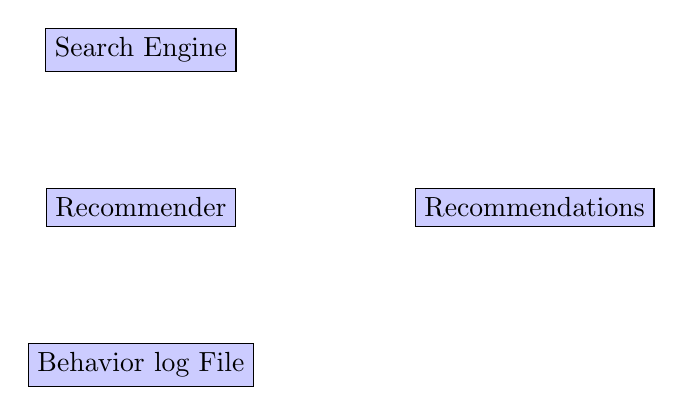
\begin{tikzpicture}[node distance=20mm,
data/.style={
rectangle,
draw,
thin,
fill=blue!20
}]
\node (recommender) [data] {Recommender};
\node (topn) [data,right of = recommender, node distance=50mm] {Recommendations};
\node (history) [data,below of = recommender] {Behavior log File};
\node (db) [data,above of= recommender] {Search Engine};
\end{tikzpicture}
\caption{Recommender engine}
\end{figure}

The described design has the following benefits
\begin{itemize}
\item Exploit existing search engine technology.
\item The search engine can be used for conventional search as well.
\item Users can use search engine to search for metadata.
\item Recommender engine can be extended with additional indicators.
\end{itemize}

\subsection{Log-likelihood similarity}
\label{sec:llr}

In order to compute the similarity between two items we use co-occurence or the log likelihood similarity.
Co-occurence in the context of recommender systems describes the circumstance that two items are similar when the same users interact (like, purchase, etc) interact with them.

The co-occurence based recommender uses the user history in order to make recommendations. The user history doesnt contains explicit preference values. Explicit user preferences are ratings of a user for an item. The user history only contains interactions of users and items. 

We can use various user actions to compute the similarity of two items. For example:
\begin{itemize}
\item Purchase action
\item Click action
\item The user might click on a like button for evrey item
\end{itemize}

 The log-likelihood similiarity is based on the number of users (or tags) in common between two items. According to \cite{Dunning93} the log-likelihood similiarity is suitable for data that only captures the interaction and no preference between users and items. 

Compared to the Jaccard coefficient \cite{Hartung} the log-likelihood-based similarity computes higher similarites for anomalous co-occurences than for items that occur in every user history. The log-likelihood similarity  is the probability that two users share the same items due to chance. For a detailed explanation of the math involved see \cite{Dunning93}. 

We describe the log-likelihood-based similarity with a small example dataset. Suppose we analyse the following web log of user purchases represented as a table (see appendix of raw web log).

\begin{table}
\begin{center}
\begin{tabular}{rllll}
 & 101 & 102 & 103 & 104\\
1 & x & x & x & \\
2 & x &  & x & x\\
3 & x & x & x & \\
4 &  & x & x & x\\
5 & x & x & x & x\\
\end{tabular}
\end{center}
\caption{Example dataset. The columns represent the user interaction with an item. Items are named 1 - 4 and users 101 - 104}
\label{tbl:llr}
\end{table}

Table \ref{tbl:llr} shows the purchases of four users for five items. The items are represented with ids 1-4 and the users with ids 101 - 104.
In the example dataset of table \ref{tbl:llr} the items 1 and 2 are similar because they purchased the same items. 

In order to get the similarity between all items we compute the log-likelihood ratio strength for every item pair. This will produce a $5 \times 5$ indicator matrix. Table \ref{tab:indicatormatrix} shows the indicator matrix for the sample dataset from table \ref{tbl:llr}

\begin{table}
  \centering
\begin{center}
\begin{tabular}{rrrrrr}
 & 1 & 2 & 3 & 4 & 5\\
1 &  & 0.40 & 0.81 & 0.63 & 0\\
2 & 0.40 &  & 0.40 & 0.63 & 0\\
3 & 0.81 & 0.40 &  & 0.63 & 0\\
4 & 0.63 & 0.63 & 0.63 &  & 0\\
5 & 0 & 0 & 0 & 0 & \\
 &  &  &  &  & \\
\end{tabular}
\end{center}
  \caption{Indicator matrix for item purchases}
  \label{tab:indicatormatrix}
\end{table}


Allthoug item 5 share all users with item 1 and 3, the log-likelihood ratio is 0. Every user purchased item 5. It would not be interesting to recommend item 5 to a user because it is to obious.
\subsection{Apache Solr}
\label{sec:solr}

Solr is a search engine that is optimized to search large volumes of text-centric data and return results sorted by relevance. It is built on Apache Lucene, an information retrieval library.

A reason why we deploy a search engine is that the application is read-dominant. The recommender will query the data far more often than it will create new documents or update the indicators. Solr is optimized to for executing queries as opposed to storing data.

Solr stores the documents in a flat structure.

Solr return documents sorted in descending order by a score that indicates the strength of the match of the document to the query. In a relational database a row either mathces a query or it does not.

The reason why we deploy a search engine in order to make recommendations is that Solr scores documents based on the presence of query terms in the document similar to a recommendations engine based on the presence of indicator.

Solr is able to parse text streams. It extract the structure and make it searchable.

\subsection{Apache Spark}
\label{sec:spark}
\verb|spark-rowsimilarity| is a script that comes with spark. It takes as input a text file representation of a matrix of sparse vectors. It finds similar rows. The input is in text-delimited form where there are three delimiters used. By default it reads (rowID<tab>columnID1:strength1<space>columnID2:strength2...) The job only supports LLR similarity. This job only supports LLR similarity.
The input has the following format:
\begin{verbatim}
1	1
2	2
3	3 
\end{verbatim}


\section{Evaluation}
\label{sec:evaluation}
Recommenders answer the question "What are the best recommendations for a user?". If we want to evaluate a recommender, we have to define, what's a "good" recommendation.
Some recommender predict the preferences of a user. One possibility to evaluate a recommender is to calculate the difference between the estimated preference and the actual preference.

Those actual prefences don't exist. Nobody knows how a user likes some new item in the future.
But we can simulate the prefencences of the future by setting aside a small part of the real data set as test data. These preferences aren't present in the training data set. Instead the recommender predicts the preferences for the missing test data set and the estimates are compared to the actual values.

Another approach to evaluate a recommender is to take a broader view of the recommender problem. It's not strictly necessary to estimate preference values in order to produce recommendations. In many cases presenting a ordered list of recommendations is sufficient. The list is ordered from best to worst recommendation.


\subsection{Dataset}
\label{sec:dataset}

This dataset used in this project describes rating and free-text tagging activity from MovieLens, a movie recommendation service \cite{movielensdata}.
MovieLens data sets were collected by the GroupLens Research Project at the University of Minnesota.
 
This data set consists of:
\begin{itemize}
\item 100,000 ratings (1-5) from 943 users on 1682 movies. 
\item Each user has rated at least 20 movies. 
\end{itemize}

The data was collected through the MovieLens web site (movielens.umn.edu) during the seven-month period from September 19th, 
1997 through April 22nd, 1998.

All selected users had rated at least 20 movies.
All ratings are contained in the file ratings.csv. Each line of this file after the header row represents one rating of one movie by one user, and has the following format:

\begin{verbatim}
userId,movieId,rating,timestamp.
\end{verbatim}

All tags are contained in the file $tags.csv$. Each line of this file after the header row represents one tag applied to one movie by one user, and has the following format:
\begin{verbatim}
userId,movieId,tag,timestamp
\end{verbatim}

\subsection{Movielens}
\label{sec:movielens}

The MovieLens dataset describes 5-star rating and free-text tagging activity from MovieLens, a movie recommendation service. It contains 100023 ratings and 2488 tag applications across 8570 movies. These data were created by 706 users 


\subsection{Precision and Recall}
\label{sec:precision}


\begin{description}
\item[Precision] Precision is the proportion of top results that relevant. Suppose the recommender recommends 5 items. If 3 items are good recommendations then the precision is $3/5$.
\item[Recall] Recall is the proportion of good recommendations that appear in the recommendation result. Suppose there are 9 good recommendations. If the recommender results contains 3 of these good recommendations then the recall is 3/9.
\end{description}

In order to calculate precision and recall the implementation determines the top \verb|n| preferences for each user. It removes those preferences from the data model. It evaluates precision and recall with the new data model. It calculates a top-N recommendation list for each user and compares it with the real top-N preferences.

The evaluation process has the following paramters:
\begin{description}
\item[Size of the result] The number of recommendations to consider. The length of the recommendation list.
\item[Relevance] Determines if an item is relevant or not.
\end{description}


\subsection{Baseline Algorithm}
\label{sec:baselinealgorithm}


\section{Multimodalrecommender}
\label{sec:multimodalrecommender}

The recommender has the follwowing parameters:
\begin{itemize}
\item The number of ratings or tags that are used for the query.
\end{itemize}

\subsection{Results}
\label{sec:results}


\subsection{Example data set}
\label{sec:exampledataset}

The example data set is a small set of user preferences. It has constructect properties:
\begin{itemize}
\item Items 108, 109 und 111 are similiar.
\item User 9 likes the items 111, 109 

\end{itemize}

\section{Conclusion}
\label{sec:similarity}

A large amount of work was required to convert formats between the user logs the Apache Mahout and Apache Solr.

\section{Infrastructur}
\label{sec:infrastructur}

\appendix

\section{Sample Input Data}
\label{sec:sampleinput}

\begin{verbatim}
itemid, userid, timestamp
1,101,980730861
1,102,980731380
1,103,980731926
2,101,980732037
2,103,980730408
2,104,980731766
3,101,980731282
3,102,980730769
3,103,980731208
4,102,980732235
4,103,980731417
5,101,980731745
5,102,980731621
5,103,980731417
5,104,980731208
\end{verbatim}

\section{Case Study: artoffer.ch}
\label{sec:artoffer}

The following action are used as indicators
\begin{itemize}
\item When a user visits the page of a item. (boolean)
\item When a user likes an item.
\item Tags
\end{itemize}
\bibliographystyle{plain}
\bibliography{a}
\end{document}
